\documentclass[12pt]{article}

\title{Progetto di sistemi complessi}
\author{Simone Balducci, Alessandro Mancini}
\date{}

\usepackage{amsmath}
\usepackage{amsfonts}
\usepackage{amssymb}
\usepackage{amsthm}
\usepackage{braket}
\usepackage{bbold}
\usepackage[margin=2cm]{geometry}
\usepackage{pgfplots}
\usepackage{fancyhdr}
\usepackage{physics}
\usepackage{systeme,mathtools}
\usepackage{graphicx}
\graphicspath{{./}}
\usepackage{float}
\usepackage{relsize}
\usepackage{dsfont}
\usepackage{calligra}
%\usepackage{siunitx}
\usepackage{circuitikz}
\usepackage[miktex]{gnuplottex}
\usepackage{epstopdf}
\usepackage[italian]{babel}
\usepackage{float}


\newcommand{\vv}{\vec{v}}
\newcommand{\vw}{\vec{w}}
\newcommand{\vov}{\vec{0_V}}
\newcommand{\vow}{\vec{0_W}}
\newcommand{\vo}{\vec{0}}
\newcommand{\vx}{\vec{x}}
\newcommand{\R}{\Re}
\newcommand{\la}{\lambda}
\newcommand{\bd}{\textbf}
\newcommand{\lang}{\left\langle}
\newcommand{\rang}{\right\rangle}
\newcommand{\lbra}{\left\lbrace}
\newcommand{\rbra}{\right\rbrace}
\newcommand{\ih}{\hat{i}}
\newcommand{\jh}{\hat{j}}
\newcommand{\kh}{\hat{k}}
\newcommand{\nnabla}{\vec{\nabla}}
\newcommand{\vr}{\vec{r}}
\newcommand{\vac}{\vec{a}}
\newcommand{\vf}{\vec{F}}
\newcommand{\vp}{\vec{p}}
\newcommand{\vom}{\vec{\omega}}
\newcommand{\val}{\vec{\alpha}}
\newcommand{\vsr}{\vec{\mathlarger{\mathlarger{\mathlarger{\scriptr}}}}}
\makeatletter
\newcommand*\bigcdot{\mathpalette\bigcdot@{.5}}
\newcommand*\bigcdot@[2]{\mathbin{\vcenter{\hbox{\scalebox{#2}{$\m@th#1\bullet$}}}}}
\makeatother
\def\dbar{{\mathchar'26\mkern-12mu d}}
\DeclareMathAlphabet{\mathcalligra}{T1}{calligra}{m}{n}
\DeclareFontShape{T1}{calligra}{m}{n}{<->s*[2.2]callig15}{}
\newcommand{\scriptr}{\mathcalligra{r}\,}
\newcommand{\boldscriptr}{\pmb{\mathcalligra{r}}\,}

\begin{document}

\maketitle 
\section{L'oscillatore di Van Der Pol}
\subsection{Descrizione}
L'oscillatore di Van Der Pol è un sistema dinamico composto da un oscillatore smorzato, descritto dalla seguente equazione:
\begin{equation}
	\ddot{x} - \mu(1-x^2)\dot{x} + x = 0
\end{equation}
dove $x(t)$ indica l'oscillazione nello spazio delle configurazioni in funzione del tempo e $\mu$ è una costante che indica lo smorzamento. Il termine di mezzo dell'equazione è quello responsabile dello smorzamento, e quindi dell'attrito. 
\begin{figure}[h]
	\begin{center}
		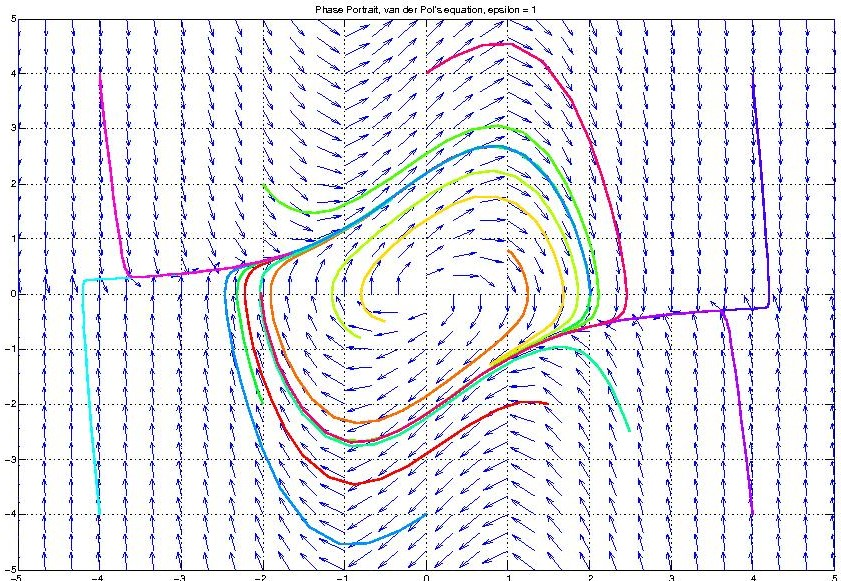
\includegraphics[scale=.5]{Spazio delle fasi oscillatore} 
		\caption{Questa figura mostra traiettorie caratteristiche dell'oscillatore di Van Der Pol nello spazio delle fasi per vari punti iniziali. Si noti anche che l'orientamento del campo vettoriale indirizza tutti i punti materiali verso la stessa traiettoria limite.}
	\end{center}
\end{figure}
Si nota subito che nel caso in cui la costante di smorzamento $\mu$ abbia valore nullo, si ottiene un oscillatore armonico classico, e questo verrà verificato nelle sezioni successive mediante simulazioni al computer e esperimenti mediante circuiti elettronici. 
\paragraph{Studio dell'equazione differenziale \\}
Consideriamo l'equazione (1) e riscriviamola come:
\begin{equation}
	\ddot{x}+\mu(x^2-1)\dot{x} = \frac{d}{dt}\left(\dot{x}+\mu\left(\frac{1}{3}x^3-x\right)\right) = \frac{d}{dt}\left(\dot{x} + \mu F(x)\right)
\end{equation}
definiamo quindi una nuova variabile
\begin{equation}
	w = \dot{x} + \mu F(x)
\end{equation}
avente derivata 
$$
	\dot{w} = -x
$$
Si ottiene quindi il sistema di equazioni
\begin{equation}
	\begin{cases}
		\dot{x} = w - \mu F(x) \\
		\dot{w} = -x
	\end{cases}
\end{equation}
Studiamo il caso $\dot{x} = 0$, che risulta in
\begin{equation}
	w(x) = \mu F(x) = \mu\left(\frac{1}{3}x^3-x\right)
\end{equation}
e si ottiene quindi una cubica. Studiamo quindi il grafico di questa funzione: 
\begin{figure}[H]
    \centering
    \begin{gnuplot}[terminal = epslatex, terminaloptions = color, terminaloptions = {size 17cm,13cm}]
        set xrange [-3:3]
        set yrange [-2.5:2.5]
        set key top left
        set key box opaque
        set key spacing 1.5
        
        plot (x*x*x)/3 -x title "F(x)" lc 7 lw 2.5, "VecField.dat" using 1:2:($3/50):($4/2) w vectors title "Campo vettoriale" lc 8 lw 0.5
    \end{gnuplot}
    \caption{Caption}
\end{figure}
Vediamo che $\dot{w} = 0$ solo per $x=0$, ovvero quando siamo sull'asse delle $y$, e si trova in particolare che sopra l'asse delle $x$ i vettori del campo vettoriale puntano a destra, mentre sotto l'asse delle $x$ puntano a sinistra. Il punto di massimo locale della funzione è $\left(-1,\frac{2}{3}\mu\right)$, mentre il punto di minimo locale è $\left(1,-\frac{2}{3}\mu\right)$. In più vediamo che i punti di intersezione tra le orizzontali che passano per i punti di massimo e minimo con la curva $w$ sono rispettivamente $\left(2,\frac{2}{3}\mu\right)$ $\left(-2,-\frac{2}{3}\mu\right)$. \\
Se consideriamo valori di $\mu$ molto più grandi di 1, vediamo che sarebbe ragionevole riscalare di nuovo le variabili:
\begin{equation}
	y = \frac{w}{\mu} \ \ \Longrightarrow \ \ \begin{cases}
		\dot{x} = \mu(y - F(x)) \\
		\dot{y} = -\frac{1}{\mu}x	
	\end{cases}
\end{equation}
Così si ottiene un grafico uguale a quello di prima ma senza i valori di $\mu$. \\
Fuori dalla curva $\dot{x} = 0$ si ha che $\dot{x}$ è molto grande, mentre $\dot{y}$ è quasi nullo. Questo vuole dire che se mettiamo una particella fuori dalla curva, questa verrà spostata orizzontalmente molto velocemente fino a posizionarsi sulla curva, e subirà anche una piccola accelerazione verticale nella direzione verso la curva. A questo punto la particella si muoverà lentamente sulla curva fino a uno dei vue punti critici, e una volta raggiunti accelererà molto velocemente fino al secondo, in corrispondenza del quale si muoverà molto più lentamente. \\
Si ottiene così un ciclo limite in cui la velocità della particella varia continuamente. In particolare notiamo che più il valore di $\mu$ è grande, più la curva si muoverà lentamente vicino ai punti di minimo/massimo e velocemente lontano da essi. Questo spiega la forma delle traiettorie viste nelle figure $$ a $$ e sarà inoltre dimostrato visivamente con delle animazioni.
\subsubsection{Studio della stabilità}
Per studiare la stabilità dell'oscillatore di Van Der Pol e la dipendenza della stessa dalla costante di smorzamento $\mu$, si usa il metodo di Lyapunov: \\ \\
\textbf{Primo teorema di Lyapunov: \\}
Per un sistema descritto da un'equazione del tipo 
\begin{equation}
	\dot{\vec{x}} = f(\vec{x},t)
\end{equation}
dove $f(\vo,t) = \vo$ per tutti i $t \geq t_0$, se esiste una funzione scalare $V(\vec{x},t)$ avente derivate parziali continue e che sottisfa le condizioni: 

1) $V(\vec{x},t)$ è definita positiva. 

2) $\dot{V}(\vec{x},t)$ è definita negativa. \\
allora il punto di equilibrio è stabile asintoticamente. \\ \\
Applichiamo ora questo teorema al caso dell'oscillatore di Van Der Pol.  \\
Prima di tutto definiamo una nuova variabile $y = \dot{x}$, in modo da passare da una singola equazione differenziale di secondo ordine a un sistema di due equazioni di primo ordine:
\begin{equation}
	\begin{cases}
		y = \dot{x} \\
		\dot{y} = \mu(1-x^2)y - x
	\end{cases}
\end{equation}
Queste equazioni rappresentano le equazioni del moto dell'oscillatore nello spazio della fasi e possono essere usate per trovare numericamente le traiettorie limite, come si vedrà nella sezione 2. \\
Consideriamo ora una funzione $V(\vec{x},t)$ del tipo 
\begin{equation}
	V(\vec{x},t) = \frac{1}{2}(x^2 + y^2)
\end{equation}
Questa funzione rispetta la prima caratteristica richiesta dal teorema di Lyapunov, ovvero è definita positiva. Si nota che la costante $1/2$ non era strettamente necessaria, ma è stata aggiunta perchè facendo la derivata totale rispetto al tempo di $V$, questa costante si semplifica e si ritrova il termine dissipativo dell'equazione (1). \\
Ora calcoliamo la derivata della funzione $V$:
$$
	\dot{V}(\vec{x},t) = x\dot{x} + y\dot{y} = x\dot{x} + \mu(1-x^2)\dot{x}^2-x\dot{x} = \mu(1-x^2)\dot{x}^2
$$
\begin{equation}
	\dot{V}(\vec{x},t) = \mu(1-x^2)\dot{x}^2
\end{equation}
Vediamo che in prossimità dell'origine questa funzione è definita negativa se e solo se $\mu$ è negativo. \\
Ne concludiamo quindi che per valori negativi di $\mu$ l'origine è un punto di equilibrio asintotico, e si dice quindi punto attrattivo. \\
Dallo studio della stabilità dell'oscillatore con il metodo di Lyapunov si trova che: 

-Se $\mu>0$, si ha che l'origine è un punto instabile e la particella si allontana da esso, fino ad arrivare su una traiettoria limite che è stabile. Si dice quindi che quella traiettoria è attrattiva. 

-Se $\mu<0$, si ha che l'origine è un punto attrattivo, quindi le traiettorie subiscono una degenerazione attorno ad essa. \\
\begin{center}
	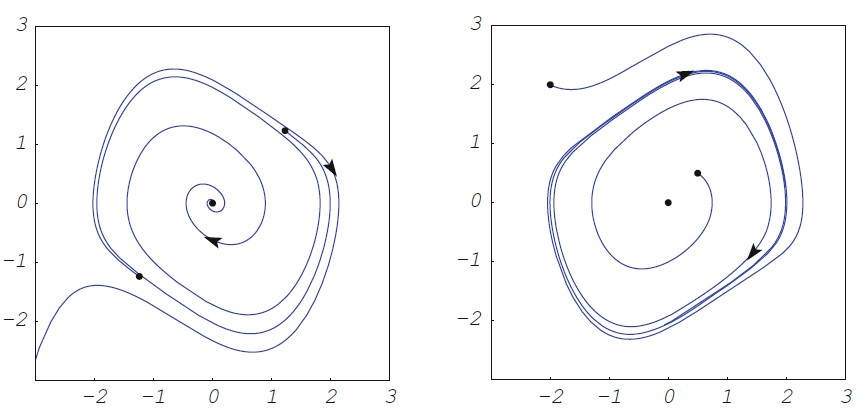
\includegraphics[scale=0.7]{Traiettorie}
\end{center}
Per valori di $\mu$ positivi, ovvero per cui si hanno delle traiettorie limite che attraggono i punti nello spazio delle fasi, si nota che l'ambiezza di queste curve cresce con lo smorzamento. \\
Come accennato in precedenza, nel caso particolare in cui $\mu = 0$, il sistema si riduce a un oscillatore armonico, quindi la traiettoria sarà una circonferenza.
\begin{center}
	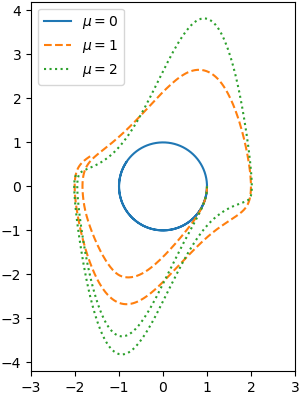
\includegraphics[scale=1]{Vari smorzamenti} 
\end{center}
\subsection{Storia}
L'oscillatore di Van Der Pol è stato ideato originariamente dall'ingegnere elettrico olandese Balthasar Van Der Pol. Van Der Pol scoprì delle oscillazioni stabili, che in seguito chiamò rilassamento-oscillazioni e che sono un tipo ci ciclo limite nei circuiti elettrici che utilizzano i vacuum tubes. \\
Quando questi circuiti venivano portati vicino al ciclo limite, questi diventavano sincronizzati, ovvero il segnale portante trasportava con se anche la corrente. \\
Van Der Pol e i suoi colleghi scoprirono inoltre che a certe frequenze si sentiva un rumore irregolare, che più avanti verrà attribuito al caos deterministico. 
\subsection{Applicazioni}
\subsubsection{Applicazioni ingegneristiche }
\subsubsection{Il neurone}
\subsubsection{Il modello di Fitzhugh-Nagumo }
Il modello di FitzHugh-Nagumo è un modello che descrive il prototipo di un sistema eccitabile, ad esempio un neurone. \\
Questo modello fornisce un ulteriore esempio delle "relaxation-oscillations", perchè se lo stimolo esterno supera un certo valore di soglia, il sistema esibirà una certa traiettoria nello spazio delle fasi prima che le variabili tornino ai valori iniziali. \\
Le equazioni che descrivono il modello sono:
\begin{equation}
	\begin{cases}
		\dot{v} = v - \dfrac{v^3}{3} - w + RI_{ext} \\
		\tau \dot{w} = v + a - bw
	\end{cases}
\end{equation}
dove $v$ è il potenziale di membrava, $w$ è la variabile di recupero e $I_{ext}$ è il modulo dell'impulso esterno. \\
La tensione di membrana $v$ è una variabile non lineare, che permette auto-eccitazioni mediante un feedback positivo, mentre $w$ è una variabile di recupero, avente dinamica non lineare che produce un feedback negativo più lento. \\
Un'importanze differenza tra queste due variabili è quindi il fatto che la $v$ abbia una dinamica veloce, mentre la dinamica di $w$ è molto più lenta. \\
E' possibile astrarre il modello "nascondendo" l'andamento non lineare della $v$ dentro una funzione $f(v)$, che è un generico polinomio di terzo grado:
\begin{equation}
	\begin{cases}
		\dot{v} = f(v) - w + I_{ext} \\
		\dot{w} = a(bV - cW)
	\end{cases}
\end{equation} 
dove $a$, $b$ e $c$ sono parametri costanti. \\
FitzHugh modificò il modello di Van Der Pol per spiegare proprietà basilari di eccitabilità esibite nelle equazioni di Hodkin-Huxley. Le nullcline nell'oscillatore di Van Der Pol erano una retta vertiale e una cubica, che si intersecavano in un singolo punto che era sempre instabile. \\
In modo da rappresentare un vero neurone, questo nuovo modello deve avere un punto critico che sia stabile, e deve anche presentare un fenomeno di soglia per un cambio di parametro che dovrebbe ricordare una stimolazione di corrente. Si può ottenere l'aggiunta di questo punto stabile aggiungendo un termine lineare $cW$ alla seconda equazione $$a$$ (in realtà si otterrebbe lo stesso effetto aggiungendo un'altro termine lineare nella prima equazione). \\
Il termine costante $c$ serve per assicurarsi che il punto critico, in condizioni di stimolazione nulla ($I_{ext} = 0$), stia sul ramo ascendente e sia stabile. \\
La dinamica di questo sistema si può immaginare come una particella che salta a destra e a sinistra dei rami della cubica. \\ \\
Questo modello è una versione semplificata in 2D del modello di Hodgkin-Huxley, che modella in dettaglio la dinamica di attivazione e disattivazione di un neurone. Tale modello è più realistico e accurato del modello di Fitzhugh-Nagumo, ma essendo un modello con traiettorie di fase quadridimensionali è difficilmente osservabile e si possono solo osservare le proiezioni delle traiettorie. La semplicità del modello di Fitzhugh-Nagumo invece permette di vedere tutte le soluzioni, e questo permette di spiegare geometricamente molti importanti fenomenti biologici legati all'eccitazione di un neurone con un meccanismo di generazione a "spike". \\ \\
\subsection{Varianti: L'oscillatore di Van Der Pol forzato}

\section{Soluzione numerica e simulazione}
Per risolvere l'equazione differenziale dell'oscillatore è stato scritto un codice in C++, che ha permesso di trovare i valori di $x$ per dei valori di tempo discretizzati $t = n\Delta$. Per fare ciò si è partiti dall'equazione 2, ma per permettere al computer di interpretarla la si è dovuta discretizzare, ottenendo il seguente sistema:
\begin{equation}
	\begin{cases}
	x_{n+1} = x_n + y_n\Delta \\
	y_{n+1} = y_n + \left(\mu(1-x_n^2)y_n - x_n\right)\Delta
	\end{cases}
\end{equation} 
Sulla base di queste equazioni discretizzate è stato scritto il codice, che per comodità è stato riportato nell'appendice in fondo al documento. \\ \\ 
Come di vede, questo codice prende come parametri di entrata le coordinate iniziali $x_0$ e $y_0$, il parametro di smorzamento $\mu$ e lo step temporale $\Delta$. L'ultimo parametro è il tempo $t$, e scegliendo questo valore si ottengono i valori della $x$ per ogni istante temporale precedente al $t$ scelto. \\
Mediante questo codice vogliamo osservare certe caratteristiche dell'oscillatore: \\
1) Vogliamo osservare la traiettoria caratteristica di un punto nello spazio delle fasi. \\
2) Vogliamo confrontare traiettorie diverse con stesse coordinate iniziali ma con diversi valori del parametro di smorzamento. \\
3) Vogliamo osservare un comportamento particolare del modello di Van Der Pol, ovvero che se prendiamo un insieme di tanti punti distribuiti in modo casuale nello spazio delle fasi, dopo poche iterazioni questi seguono tutti la stessa traiettoria, che è quindi una curva attrattrice. \\
4) Vogliamo infine osservare l'andamento temporale della posizione $x$ della particella. \\
Partiamo dal primo obiettivo, ovvero la traiettoria carattestistica: 
\begin{figure}[H]
    \centering
    \begin{gnuplot}[terminal=epslatex, terminaloptions=color, terminaloptions={size 14cm, 12cm}]
        set xlabel "x"
        set ylabel "p"
        set key top left
        set key box
        set key spacing 1.5
        set grid

        plot "VDP15.dat" title "µ = 1.5" pt 7 lc 2
    \end{gnuplot}
\end{figure}
Nella figura soprastante si può vedere la traiettoria caratteristica dell'oscillatore di Van Der Pol. Come è stato spiegato nelle sezioni precedenti, la velocità del punto che si muove secondo questa traiettoria non è affatto costante.
Come si può notare dall'animazione infatti, il punto si muove molto più velocemente nei lati corti della traiettoria e più lentamente nei lati lunghi. Si avrà quindi un accumulo di punti in corrispondenza dei punti in cui il momento cambia segno,
che nel grafico soprastante si trovano in corrispondenza dei punti $(-2,0)$ e $(2,0)$ approssimativamente. \\
Nell'immagine sottostante si può vedere uno degli ultimi frame dell'animazione citata in precedenza e si vede chiaramente che nei lati corti si hanno degli accumuli di punti, mentre lungo i lati lunghi i punti si distribuiscono in maniera molto meno densa. 
\begin{figure}[H]
	\centering
	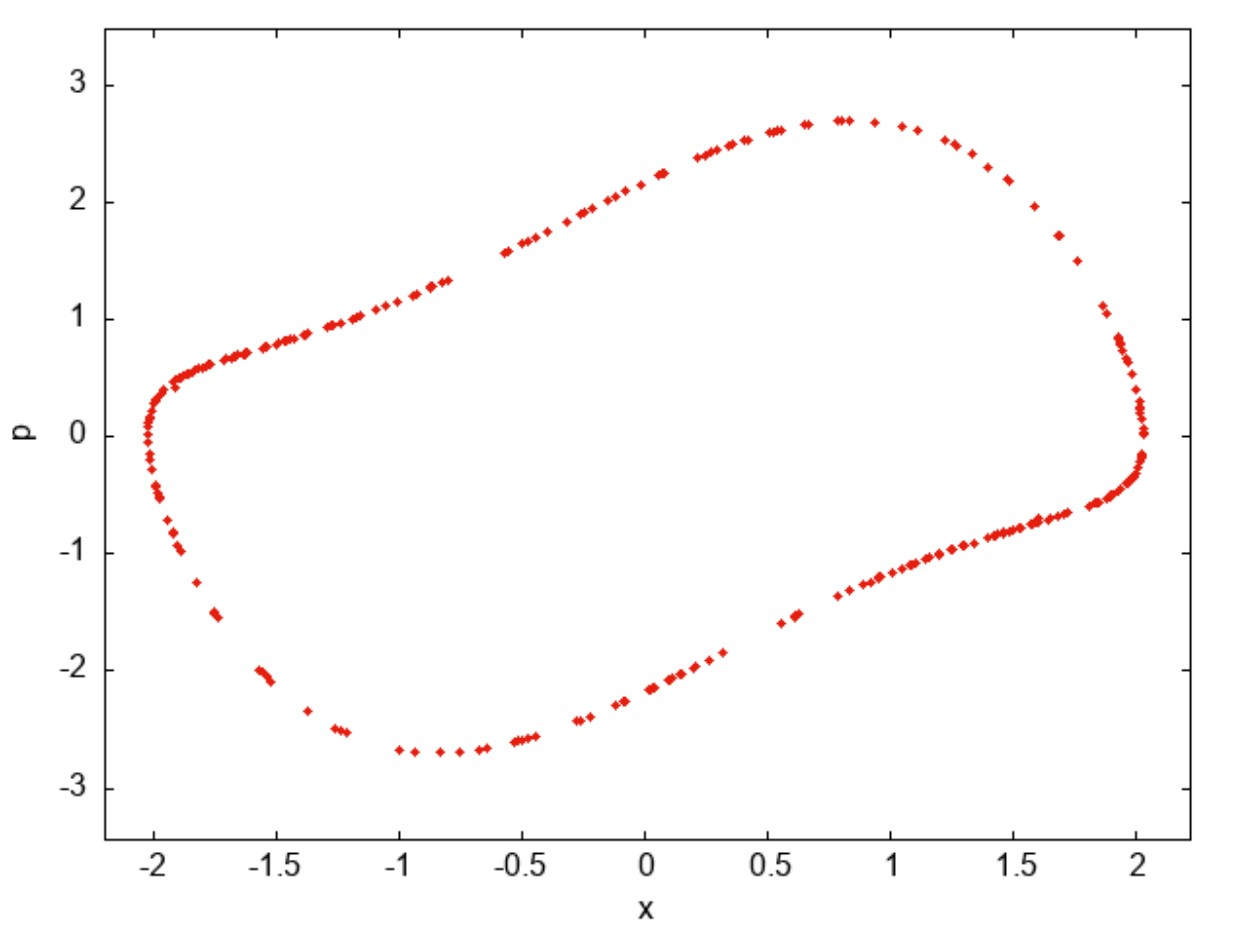
\includegraphics[scale = 0.4]{Frame animazione}
\end{figure}
Vogliamo ora confrontare le traiettorie di particelle aventi stesse coordinate iniziali ma diverse costanti di smorzamento. \\
Ci aspettiamo che il grafico ottenuto dalla simulazione numerica sia simile a quello visto in figura $$ afads $$. Dalla simulazione si ottiene il seguente grafico:
\begin{figure}[H]
	\centering
	\begin{gnuplot}[terminal = epslatex, terminaloptions = color, terminaloptions = {size 12cm,18cm}]
		set key top left
		set key box
		set key spacing 1.5
		set grid
		set ytics -6,1,6
		set yrange [-5.5:5.5]
    
		plot "VDP1.dat" title "µ = 1" pt 7 lc 2, "VDP2.dat" title "µ = 2" pt 7 lc 22, "VDP3.dat" title "µ = 3" pt 7 lc 4
	\end{gnuplot}
\end{figure}
che riporta l'andamento atteso. Studiamo questo grafico: \\
La cosa principale che si nota è che, con l'aumentare del valore di $\mu$, la traiettoria si allunga e assume una forma pià angolata. Il motivo di questo comportamento è stato spiegato nella sezione precedente e deriva dallo studio dell'equazione differenziale. \\
Vogliamo ora considerare le traiettorie in corrispondenza di valori piccoli di $\mu$.
\begin{figure}[H]
    \centering
    \begin{gnuplot}[terminal=epslatex, terminaloptions=color, terminaloptions={size 15cm, 15cm}]
		set xlabel "x"
		set ylabel "p"
		set key top left
		set key box
		set key spacing 1.5
		set grid

		plot "VDP-05.dat" title "µ = -0.5" pt 7 lc 3
    \end{gnuplot}
    \caption{Grafico ottenuto con $\mu = -0.5$}
\end{figure}
Nel grafico soprastante si vede che la particella parte vicino all'origine e viene attratta verso essa, percorrendo quindi delle orbite che degenerano fino a collassare in un punto.
Vogliamo ora studiare un comportamento molto interessante di questo tipo di oscillatore che è stato accennato nelle pagine precedenti. \\
Consideriamo una situazioni iniziale come quella nel grafico seguente
\begin{figure}[H]
    \centering
    \begin{gnuplot}[terminal=epslatex, terminaloptions=color, terminaloptions={size 15cm, 15cm}]
    set xlabel "x"
    set ylabel "p"
    unset key
    set grid
    set xrange [-2:2]
    set yrange [-2:2]

    plot "Animazione_frame_1.dat" pt 7 lc 7
    \end{gnuplot}
    \caption{Frame iniziale dell'animazione.}
\end{figure}
quindi una situazione in cui abbiamo un grande numero di punti (in questo caso ne sono stati plottati 300) che sono distribuiti randomicamente nello spazio delle fasi, quindi con momento iniziale e coordinata $x$ iniziale randomici. \\
Se lasciamo partire questi punti, sembra inizialmente che questi si muovano in modo caotico, ma dopo una decina di iterazioni si vede che le particelle stanno in realtà andando a formare una stessa traiettoria, che è la traiettoria caratteristica dell'oscillatore di Van Der Pol. \\
In base alla loro posizione iniziale i punti ci metteranno più o meno tempo a posizionarsi su questa curva, ma dopo un numero sufficientemente grande di iterazioni (nella simulazione considerata sono servite circa 350 iterazioni) tutti i punti si saranno posizionati sulla curva. \\
Questo comportamento peculiare è un'altra dimostrazione del fatto che la traiettoria dell'oscillatore di Van Der Pol sia una curva attrattiva. \\ \\
Infine si vuole studiare l'andamento temporale della $x$.
\begin{figure}[h]
    \centering
    \begin{gnuplot}[terminal = epslatex, terminaloptions = color, terminaloptions = {size 18cm,12cm}]
        set key box opaque
        set grid 
        set key spacing 1.5
        set xlabel "t"
        set ylabel "x(t)"
        set ylabel offset 1
        
        plot "AndTemp.dat" title "Andamento temporale" pt 7 lc 22
    \end{gnuplot}
    \caption{Grafico che mostra l'andamento temporale delle oscillazioni della grandezza $x(t)$.}
\end{figure}
Nella figura soprastante si vede che l'andamento della $x$ ricorda vagamente una sinusoide, per la periodicità, ma ha una forma molto più aguzza. Si nota inoltre che la forma della funzione tra un punto di minimo e un punto di massimo e viceverda mantiene la stessa forma, ma risulta capovolta. \\
La forma di queste oscillazioni cambia molto con il valore della costante di smorzamento. Infatti si trova che per valori più piccoli di $\mu$ le oscillazioni hanno una forma più aguzza, mentre per valori grandi (da circa 5 in su)l'andamento ha una forma più squadrata. \\
Per rendere l'idea in un modo tutt'altro che rigoroso, per valori piccoli di $\mu$ l'andamento ha una forma che ricorda il dente di un lupo, mentre per valori grandi ha una forma che ricorda il dente di uno squalo. \\ \\ 
Questo è l'andamento temporale nel caso dell'oscillatore non forzato. \\
Per un oscillatore forzato si troverebbe un andamento vagamente simile a questo, ma con una forma molto più irregolare. Questo è dovuto al fatto che in un'oscillatore del genere, una forzante periodica producerebbe una caoticità, che renderebbe quindi molto più imprevedibile la traiettoria.
\section{Circuito elettronico}

\section{Bibliografia}


\end{document}
